\documentclass{beamer}
%
% Choose how your presentation looks.
%
% For more themes, color themes and font themes, see:
% http://deic.uab.es/~iblanes/beamer_gallery/index_by_theme.html
%
\mode<presentation>
{
  \usetheme{Boadilla}      % or try Darmstadt, Madrid, Warsaw, ...
  \usecolortheme{beaver} % or try albatross, beaver, crane, ...
  \usefonttheme{default}  % or try serif, structurebold, ...
  \setbeamertemplate{navigation symbols}{}
  \setbeamertemplate{caption}[numbered]
  
} 

\usepackage{xcolor,colortbl}
\usepackage[english]{babel}
\usepackage[utf8x]{inputenc}
\usepackage{courier}
\usepackage{dsfont}
\usepackage{verbatim} 
\usepackage{enumerate}
\usepackage{tikz}
\usepackage{multirow}
\usepackage{venndiagram}
\usepackage{epigraph} 
%\usepackage{xcolor}

%\usepackage{enumitem}

\usepackage{hyperref}
\hypersetup{
    colorlinks=true,
    linkcolor=blue,
    filecolor=magenta,      
    urlcolor=cyan,
}

\usetikzlibrary{shapes,decorations,arrows,calc,arrows.meta,fit,positioning}
\tikzset{
    -Latex,auto,node distance =1 cm and 1 cm,semithick,
    state/.style ={ellipse, draw, minimum width = 0.7 cm},
    point/.style = {circle, draw, inner sep=0.04cm,fill,node contents={}},
    bidirected/.style={Latex-Latex,dashed},
    el/.style = {inner sep=2pt, align=left, sloped}
}

\setbeamertemplate{enumerate items}[default]

%\setitemize{label=\usebeamerfont*{itemize item}%
%  \usebeamercolor[fg]{itemize item}
%  \usebeamertemplate{itemize item}}

\newcommand{\Mypm}{\mathbin{\tikz [x=1.4ex,y=1.4ex,line width=.1ex] \draw (0.0,0) -- (1.0,0) (0.5,0.08) -- (0.5,0.92) (0.0,0.5) -- (1.0,0.5);}}%

\title[STA-209]{Visualizing Data}
\subtitle{}
\author{Grinnell College}
\date{September 6, 2024}

\begin{document}

\begin{frame}
  \titlepage
  \centering Nathan Friedrichsen
\end{frame}

\begin{frame}{Goals for Class Today}
We are going to learn how to do the following today:

\begin{enumerate}
    \item use appropriate graphs to display and describe quantitative and categorical data
    \item describe the \textbf{distribution} of a variable
    \item make graphs that describe the relationship between 2 or more variables
\end{enumerate}
\end{frame}

\begin{frame}{Motivation}
Let's look at the Tips data seen previously. Here are 20 observations out of 244 regarding the tips given to one waiter over the course of several months in one restaurant.

\begin{table}[ht]
\tiny
\centering
\begin{tabular}{rrllllr}
  \hline
Total Bill & Tip & Sex & Smoker & Day & Time & Size \\ 
  \hline
13.42 & 1.58 & Male & Yes & Fri & Lunch &   2 \\ 
  16.27 & 2.50 & Female & Yes & Fri & Lunch &   2 \\ 
  10.09 & 2.00 & Female & Yes & Fri & Lunch &   2 \\ 
  20.45 & 3.00 & Male & No & Sat & Dinner &   4 \\ 
  13.28 & 2.72 & Male & No & Sat & Dinner &   2 \\ 
  22.12 & 2.88 & Female & Yes & Sat & Dinner &   2 \\ 
  24.01 & 2.00 & Male & Yes & Sat & Dinner &   4 \\ 
  15.69 & 3.00 & Male & Yes & Sat & Dinner &   3 \\ 
  11.61 & 3.39 & Male & No & Sat & Dinner &   2 \\ 
  10.77 & 1.47 & Male & No & Sat & Dinner &   2 \\ 
  15.53 & 3.00 & Male & Yes & Sat & Dinner &   2 \\ 
  10.07 & 1.25 & Male & No & Sat & Dinner &   2 \\ 
  12.60 & 1.00 & Male & Yes & Sat & Dinner &   2 \\ 
  32.83 & 1.17 & Male & Yes & Sat & Dinner &   2 \\ 
  35.83 & 4.67 & Female & No & Sat & Dinner &   3 \\ 
  29.03 & 5.92 & Male & No & Sat & Dinner &   3 \\ 
  27.18 & 2.00 & Female & Yes & Sat & Dinner &   2 \\ 
  22.67 & 2.00 & Male & Yes & Sat & Dinner &   2 \\ 
  17.82 & 1.75 & Male & No & Sat & Dinner &   2 \\ 
  18.78 & 3.00 & Female & No & Thur & Dinner &   2 \\ 
   \hline
\end{tabular}
\end{table}
Do more customers come to the restaurant on certain days? 

\textbf{Hard to tell by looking at table}
\end{frame}

\begin{frame}{Motivation}
Data collection has made remarkable progress in the last decades, giving us a greater quantity of data than most could ever dream of. However, just looking at tables of data is not very useful. \vspace{3mm} 

Better approaches:
\begin{enumerate}
    \item \textbf{Data Visualization} displaying data in ways that make patterns more noticeable
    \item \textbf{Numerical Summaries} calculating numbers that tell us about certain aspects of the data
\end{enumerate}
\end{frame}

\begin{frame}{Data Visualization}
    Previously, I made a big deal out of determining if a variable is categorical or quantitative \vspace{4mm}

    \textbf{Why?} Because the type of variable is going to determine how we make graphs to display and describe the data \vspace{4mm}

    The types graphs we make also will be determined by \textit{how many} different variables we are working with
\end{frame}

\begin{frame}{Distribution}
In order to better understand patterns in our data, we will often combine graphics with short descriptions of what we see. A term we will use often: \vspace{10mm}

The \textbf{distribution} of a variable refers to how frequently certain values of that variable show up in our data 
\end{frame}




\begin{frame}{One Categorical Variable}
When we have one categorical variable, a \textit{barchart} is often used to tally the frequencies (counts) of that categorical variable
\begin{center}
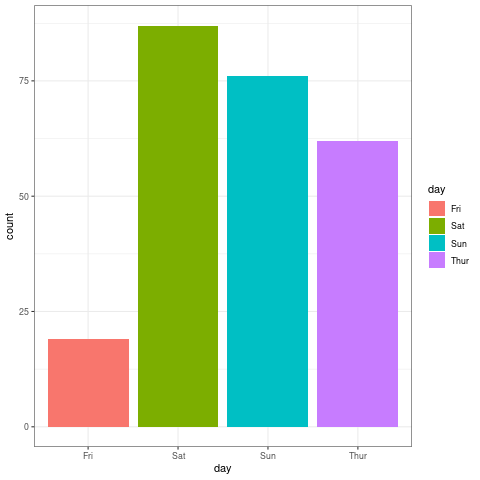
\includegraphics[scale=0.35]{img/tip_day.png}
\end{center}
\end{frame}

\begin{frame}{One Categorical Variable}
To describe the distribution of a categorical variable, we just need to talk about how likely each category is, and mention the most and least likely categories (helpful to include supporting values)


\begin{tabular}{cl}  
         \begin{tabular}{c}
           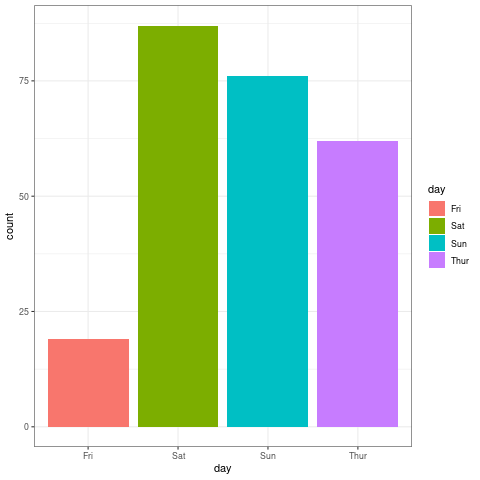
\includegraphics[scale=0.35]{img/tip_day.png}
           \end{tabular}
           & \begin{tabular}{l}
             \parbox{0.5\linewidth}{%  change the parbox width as appropiate
             \textbf{Distribution of customers?}  \vspace{20mm}
    }
         \end{tabular}  \\
\end{tabular}
    
\end{frame}


\begin{frame}{One Quantitative Variable}
For quantitative variables, a \textbf{histogram} is often used to show the distribution of values. Histograms group numeric values into equally spaced intervals known as bins, then display the frequencies/counts (or \% or proportion) of data in each bin:

\begin{center}
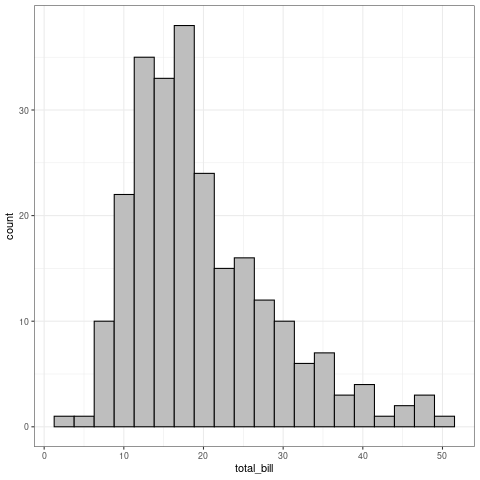
\includegraphics[scale=0.35]{img/bill_bin_20.png}
\end{center}
\end{frame}

\begin{frame}{Histogram Bin Width}
Using wider/narrower bin width can drastically change the histogram

    - too wide: can't tell exactly where data points are
    
    - too narrow: overly detailed and hard to read
\begin{center}
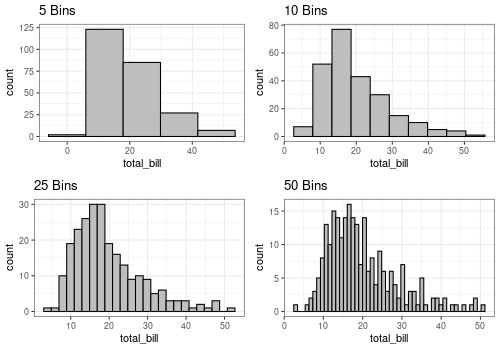
\includegraphics[scale=0.5]{img/bin_grid.png}
\end{center}
\end{frame}

\begin{frame}{One Quantitative Variable}
\begin{columns}

  \begin{column}{0.45\textwidth}
	\begin{center}
	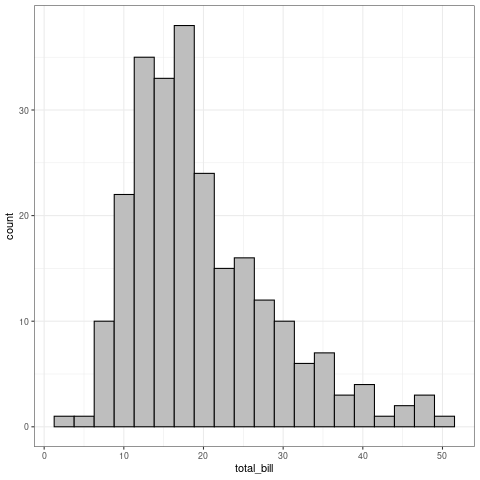
\includegraphics[scale=0.35]{img/bill_bin_20.png}
	\end{center}
  \end{column}
  \begin{column}{0.45\textwidth}
	Here, there is quite a bit more we can examine:
	\begin{itemize}
	\item Where does the ``center" appear to be?
	\item How spread out is this data?
	\item What about the range of this data?
	\item Does it appear skewed (more data on one side?)
	\end{itemize}
  \end{column}

\end{columns}
\end{frame}

\begin{frame}{One Quantitative Variable - Distribution}
Describing the \textbf{distribution} of a quant. variable is more nuanced than for a cat. variable \vspace{4mm}

We need to mention all of the following things:
\begin{itemize}%[leftmargin=1em]
 \item \textbf{Shape} - is the distribution symmetric, skewed, bell-shaped, bimodal?
 \item \textbf{Center} - where does the data bunch up (approx. mean or median)
 \item \textbf{Spread} - how spread out is the data (ie: range of values)
 \item \textbf{Outliers} - are there values that are much smaller/larger than the rest?
\end{itemize}
\end{frame}

\begin{frame}{Distribution - Shape}
\begin{center}
    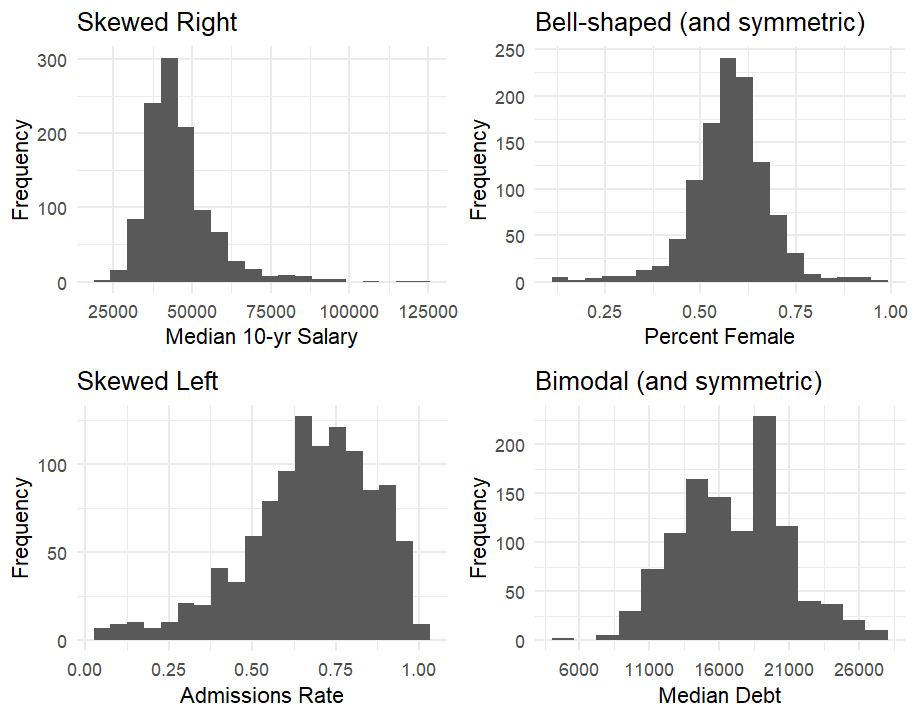
\includegraphics[scale=.6]{img/HistogramShapeExamples.png}
\end{center}
\end{frame}

\begin{frame}{Distribution - Center and Spread}
\begin{itemize}
    \item \textbf{Center}: typically we use means or medians
    \item \textbf{Spread}: typically we use standard deviation, range, or IQR
\end{itemize} \vspace{3mm}

We will talk more about how to decide which thing to use for both center and spread in a few days (and how to calculate each)  
\end{frame}

\begin{frame}{Outliers}
\textbf{Outliers} are data points that look \textit{unusual} in that they either don't follow a pattern that we see in the data or are far away from other points \vspace{3mm}

In a histogram, we identify outliers by looking for gaps in the bins
\end{frame}

\begin{frame}{Bivariate Graphs}
Up until now we have only looked at graphs that displayed one variable at a time. These are often called \textbf{univariate} graphs \vspace{3mm}

\textbf{Bivariate graphs} show the relationship between two variables
\begin{itemize}
    \item type of graph we use still depends on whether the variables are categorical or quantitative 
\end{itemize}
\begin{center}
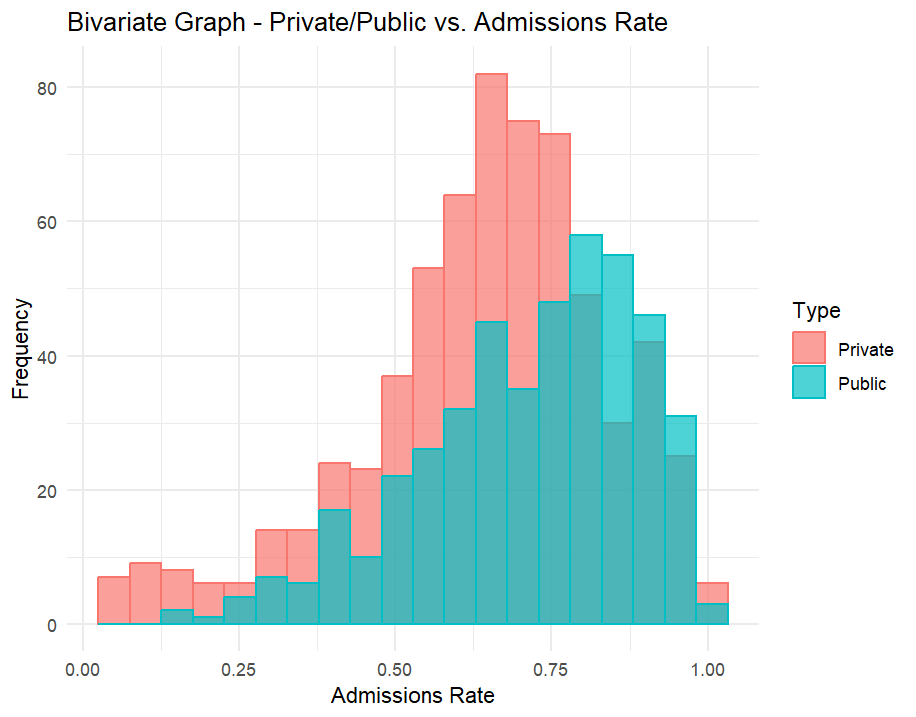
\includegraphics[scale=.4]{img/CollegeAdmissions.png}
\end{center}
\end{frame}


\begin{frame}{Association}
It is very common for us to try to find a relationship between two (or more) variables

\begin{itemize}
    \item When there seems to be some connection between two variables (knowing about one variable tells us about the other), we say they are \textbf{associated}. 
    \item If there does \underline{not} seem to be a relationship between the variables, we say they are \textbf{independent}.
\end{itemize} 
\vspace{3mm}

When discussing an association between two variables we’ll
sometimes designate an explanatory variable (suspected
cause) and a response variable (suspected effect) \vspace{3mm}

\textbf{NOTE:} this does not always mean that one variable is causing a change in the other
\end{frame}


\begin{frame}{Categorical + Categorical $\rightarrow$ Stacked Bar}
The first type of bivariate bar chart is known as a \textbf{stacked bar chart}, which allows us to break down one variable in terms of another. Here, we consider if any smokers were included in the party

\begin{center}
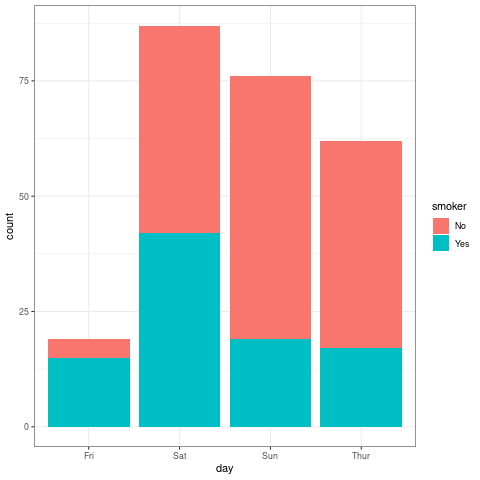
\includegraphics[scale=0.35]{img/bar_stacked.png}
\end{center}

\end{frame}

\begin{frame}{Categorical + Categorical $\rightarrow$ Dodge Bar}
The second type of bivariate bar chart is known as a \textbf{dodged bar chart}, which presents both variables alongside one another. This makes comparing within groups much simpler

\begin{center}
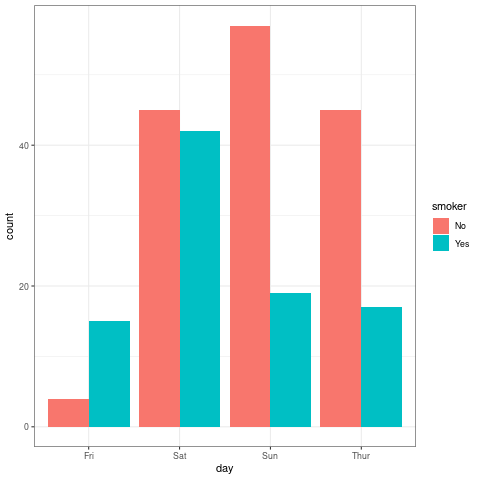
\includegraphics[scale=0.35]{img/bar_dodge.png}
\end{center}

\end{frame}

\begin{frame}{Categorical + Categorical $\rightarrow$ Filled Bar}
The last type of bivariate bar chart is known as a \textbf{filled bar chart}, offering proportions. Although we lose absolute counts, we can now see relative frequencies within each group

\begin{center}
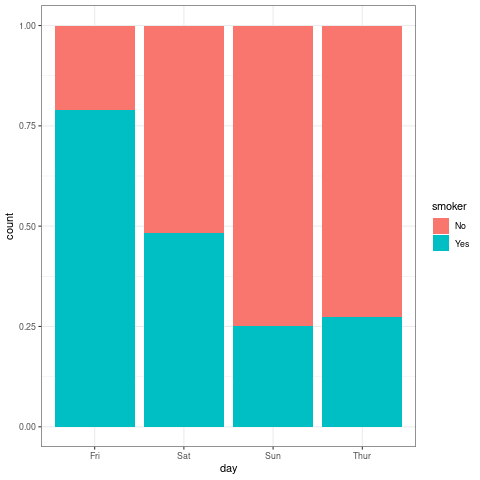
\includegraphics[scale=0.35]{img/bar_fill.png}
\end{center}
\end{frame}


\begin{frame}{Bivariate Bar Charts}
Back to the college data. Are the variables “Region” and “Type” associated? Which bar chart is most helpful?
\begin{center}
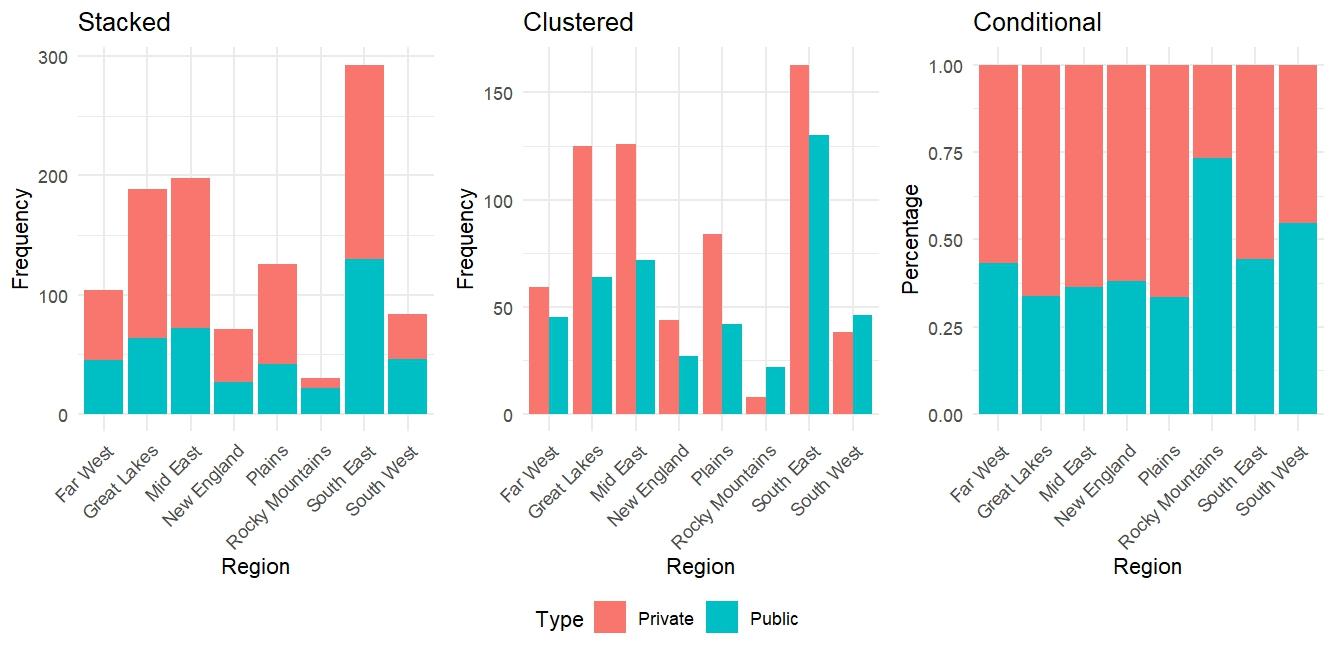
\includegraphics[scale=.5]{img/CollegeComboAssoc.jpeg}
\end{center}
\end{frame}



\begin{frame}{Quantitative + Quantitative $\rightarrow$ Scatterplots}
Visual summaries investigating the relationship between two quantitative variables are often presented with a \textbf{scatterplot} \vspace{2mm}
\begin{columns}
  \begin{column}{0.5\textwidth}
  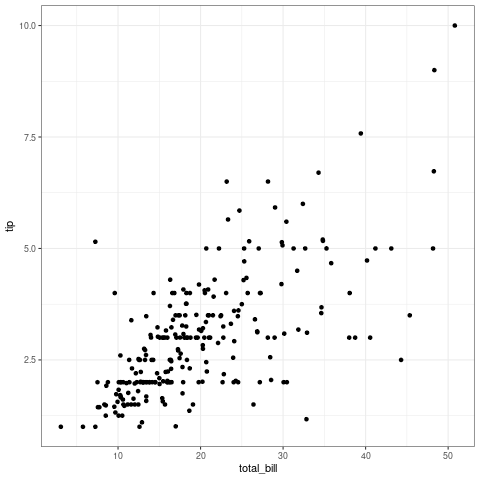
\includegraphics[scale=0.35]{img/scatter_tip.png}
  \end{column}
  \begin{column}{0.4\textwidth}
  What kind of relationship do we see between the total bill and the tip amount?
  \end{column}
\end{columns}
\end{frame}


\begin{frame}{Types of Quantitative Relationships}
\begin{center}
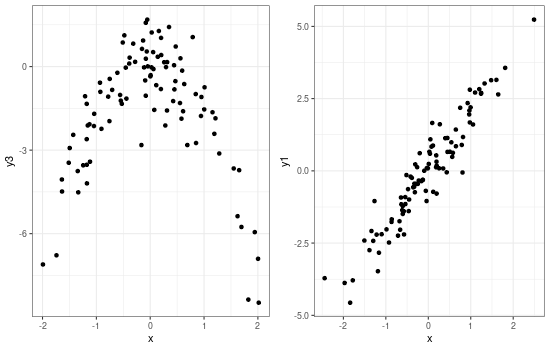
\includegraphics[scale=0.5]{img/linear_nonlinear.png}
\end{center}
\end{frame}



\begin{frame}{Types of Quantitative Relationships}
\begin{center}
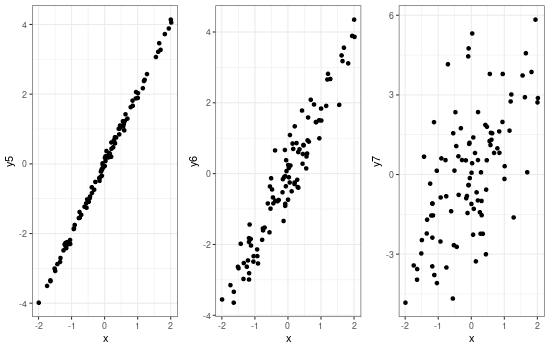
\includegraphics[scale=0.5]{img/linear_strong.png}
\end{center}
\end{frame}


\begin{frame}{Types of Quantitative Relationships}
\begin{center}
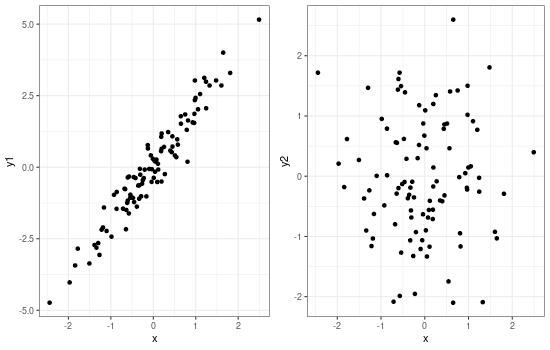
\includegraphics[scale=0.5]{img/linear_none.png}
\end{center}
\end{frame}

\begin{frame}{Describing a Scatterplot}
To describe the relationship between variables in a scatterplot we need to mention all of the following: \vspace{3mm}

\begin{itemize}
    \item \textbf{Form}: what type of pattern exists (linear / non-linear / curved)
    \item \textbf{Strength}: how close are the points? (weak / moderate / strong)
    \item \textbf{Direction}: how the values of one variable relate to the values of the other variable (positive / negative)
    \item \textbf{Outliers}
\end{itemize}
\end{frame}

\begin{frame}{Describing Scatterplots -- Example}
Canidae is the biological family that contains dogs, wolves, foxes, and similar mammals.

Two variables are bite force (N) and body mass (kg). Which would be the explanatory variable and 
which would be the response variable?

\begin{columns}
  \begin{column}{0.5\textwidth}
  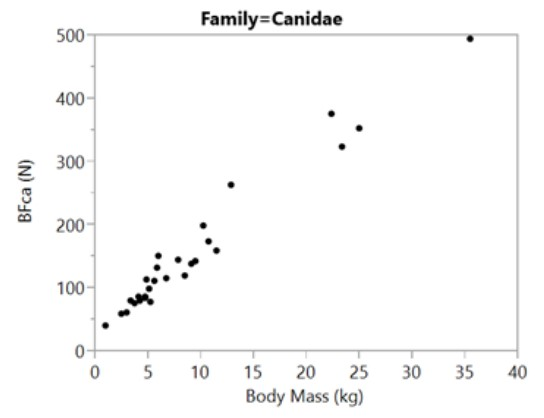
\includegraphics[scale=.65]{img/CanidaeScatterplot.jpg}
  \end{column}
  \begin{column}{0.4\textwidth}
  How do we describe the scatterplot?
  \end{column}
\end{columns}
{\tiny source: “Bite Forces and Evolutionary Adaptations to Feeding Ecology in Carnivores,” by P. Christiansen and S. Wade, Ecology, 88(2), 2007, pp. 347 – 358}

\end{frame}

\begin{frame}{Reflection}
We'll take a few minutes to reflect on what we learned. Talk with those around you to come up with answers to the following questions: \vspace{2mm}

\begin{itemize}
    \item Why do we make graphics to display data?
    \item What is the \textbf{distribution} of a variable?
    \item Why do we care about whether a variable is categorical or quantitative?
\end{itemize}
\end{frame}

\begin{frame}{Next Time}
    \begin{itemize}
        \item One other graph to display quantitative data (boxplot) \vspace{4mm}
        \item What to do when we have Quantitative + Categorical variables \vspace{4mm}
        \item Lab for putting this all into practice
    \end{itemize}
\end{frame}


\end{document}
